\documentclass[conference,10pt]{IEEEtran}
\usepackage{fancyhdr}
\usepackage{amssymb}
\usepackage{amsmath}
\usepackage{amsfonts}
\usepackage[T1]{fontenc} % get tt fonts to work right
\usepackage{graphicx}
\usepackage{multirow}
\usepackage{color}
\usepackage{caption}
\DeclareCaptionType{copyrightbox} % workaround for bug in caption
\usepackage{subcaption}
\usepackage{xspace}
\usepackage{url}

\begin{document}

\special{papersize=8.5in,11in}
\setlength{\pdfpageheight}{\paperheight}
\setlength{\pdfpagewidth}{\paperwidth}


\title{Mapping HALO Exchange onto Toruses and Stuff}

\author{\IEEEauthorblockN{
Yadu Nand\IEEEauthorrefmark{1}\IEEEauthorrefmark{2}\IEEEauthorrefmark{3},
Timothy G. Armstrong\IEEEauthorrefmark{1}}
  \IEEEauthorblockA{
  \IEEEauthorrefmark{1}Dept. of Computer Science,
    University of Chicago,
    Chicago, IL, USA}
  \IEEEauthorblockA{\IEEEauthorrefmark{2}Mathematics and Computer Science Division,
    Argonne National Laboratory,
    Argonne, IL, USA}
  \IEEEauthorblockA{\IEEEauthorrefmark{3}Computation Institute,
    University of Chicago and Argonne National Laboratory,
    Chicago, IL, USA}
}

\maketitle

 
\begin{abstract}
Abstract goes here
\end{abstract}

\section{Introduction}

Halo exchange is a commonly occurring communication pattern in parallel
codes, where each process is assigned an application subdomain and
must periodically communicate with other processors that have neighboring
subdomains to update information about the state of the boundary between
subdomains.  A common special case is when a multi-dimensional cartesian
space is decomposed into subdomains of equal size.  For example, in the
three-dimensional case, a 8x8x8 cube might be decomposed into 256 2x1x1 cubes
for execution on 256 processors.

This paper explores the problem of mapping such multi-dimensional cartesian
halo exchange communications onto parallel computers with hypercube or
torus networks.

\section{Example Section}

We're going to cite Swift/T~\cite{SwiftT_2013} and include an illustration
(see Figure~\ref{fig:task-data}). 

\label{sect:ddt-model}
\begin{figure}
  \center
  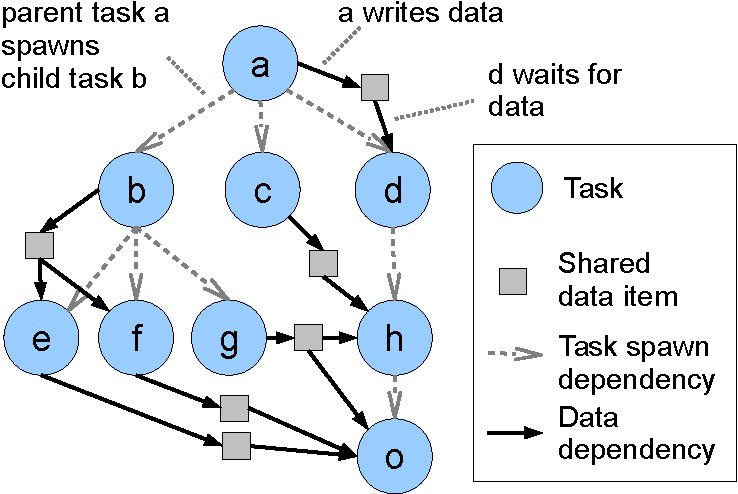
\includegraphics[width=0.325\textwidth]{fig/task-data}
  \caption{This is a figure.
    \label{fig:task-data}}
\end{figure}

\section{High-Performance Computer Networks}

\subsection{Blue Gene/Q 5D torus}
RedBook~\cite{BGQ_RedBook_2013}

\subsection{Cray Gemini 3D torus}

\section{Models for Network Communication}

\section{Experimental Design}

\section{Results}

\section{Conclusion}


\bibliographystyle{abbrv}
\bibliography{halo}

\end{document}
